\setcounter{page}{15}
\chapter{Introdução}
%apenas contexto, não tem que expor o problema
%Falar sobre a importancia e o papel da gestão/governança de TI no setor público;
A governança de Tecnologia da Informação (TI) é composta de estruturas organizacionais, processos, controles e outros componentes com objetivo de usar a TI para agregar valor ao negócio das organizações, com riscos controlados e aceitáveis. A governança de TI pode evitar ou reduzir deficiências na gestão de uma organização, tais como problemas na gestão de pessoas, em processos de planejamento, projetos e contratações \cite{weill:04,tcu:14}.

No âmbito da Administração Pública Federal\footnote{"A APF corresponde ao conjunto de órgãos da administração direta, autárquica e fundacional. Não fazem parte empresas públicas e
sociedades de economia mista." \cite{egd:16}} (APF) a governança de TI é referenciada com termos variados, como governo digital e governo eletrônico. A governança de TI na APF tem seu início na década de 2000 marcado por um projeto denominado e-Gov, cujo objetivo era priorizar o uso das tecnologias da informação e comunicação (TIC) para democratizar o acesso à informação \cite{egd:16}.

Até a presente data, o governo brasileiro vem amadurecendo seus processos de governança de TI. Destaca-se neste período a criação da Instrução Normativa número 4 (IN 04/2008), que regula as contratações de TI na APF \cite{in04:08}. No ano seguinte, em 2009, entrou em vigor um importante instrumento de governança de TI para a administração pública brasileira, a Estratégia Geral de Tecnologia da Informação (EGTI), com o objetivo de estabelecer as bases estratégicas para a melhoria da gestão de TI nos órgãos \cite{egti:08}.

Em consulta no portal da transparência do governo federal\footnote{A consulta realizada no portal da transparência na funcionalidade "Consultas por Função Orçamentária" na aba "Despesas", selecionando a finalidade "Tecnologia da Informação".} é possível verificar que, apenas no ano de 2015, as despesas com TI somam R\$ 3,445 bilhões. Diante disso, além de utilizar a tecnologia para promover serviços públicos digitais, viabilizar o acesso à informação e ampliar a participação social na construção de políticas públicas, é do interesse do governo federal administrar o orçamento destinado à TI de forma à otimizar os recursos e reduzir os riscos \cite{egd:16}.

Nos órgãos que compõem a APF o planejamento é um princípio fundamental estabelicido no Decreto Lei 200/1967. Desde o início da vigência da EGTI os órgãos do poder executivo federal são obrigados a planejar as ações que envolvem sistemas de informação (SI) e tecnologia da informação através do planejamento de TI \cite{egti:08}. Portanto, todas as organizações públicas, devem desenvolver processos de planejamento e de monitoramento nos níveis institucionais e na área de TI, permitindo assim, melhoria dos serviços de tecnologia prestados ao cidadão e melhor emprego dos orçamentos destinados à TI \cite{tcuManual:07}. 

O principal instrumento de planejamento de TI na APF, denominado Plano Diretor de Tecnologia da Informação (PDTI) é previsto como instrumento obrigatório desde a primeira versão da IN 04/2008 e da EGTI \cite{in04:08, egti:08}. O PDTI possibilita às instituições realizar o diagnóstico, planejamento e gestão dos recursos e processos de TI visando alinhamento com os objetivos estratégicos da instituição.


\section{Motivação e Caracterização do Problema}

Apesar do embasamento legal, a gestão de TI dos órgãos públicos federais não tem atendido satisfatoriamente a necessidade de planejamento. Isto é evidenciado através de uma pesquisa realizada periodicamente pelo Tribunal de Contas da União (TCU), que busca apresentar um Perfil da Governança de TI (Perfil GovTI) dos entes da APF. Os números apresentados nas pesquisas de 2007, 2010, 2012 e 2014 \cite{tcu:14} são apresentados no gráfico da Figura \ref{figura:grafico_tcu}.

\begin{figure}[h]
\centering % para centralizarmos a figura
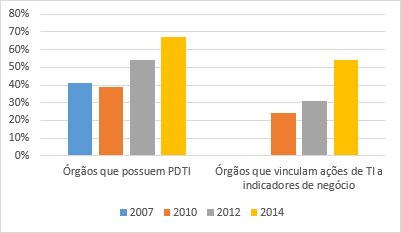
\includegraphics[width=10cm]{figuras/grafico_tcu.png}
\label{figura:grafico_tcu}
\caption{Evolução do PDTI - Perfil GovTI}
\end{figure}

Conforme ilustrado na Figura \ref{figura:grafico_tcu}, os resultados do levantamento de 2014, relatório mais recente até a presente data, apontam que 67\% dos órgãos pesquisados adotam o PDTI, ou seja, 33\% não cumprem as recomendações e determinações acerca da elaboração do PDTI. Ainda em 2014, apenas 54\% das organizações fazem o vínculo das ações de TI a indicadores e metas de negócio. O nível de adoção dessa prática é preocupante, haja vista que a TI deve existir para atender às necessidades do negócio e não dela própria. Desse modo, sem a vinculação das ações de TI aos indicadores e metas de negócio, fica difícil de avaliar a efetividade e a própria necessidade dessas ações \cite{tcu:14}. 

O TCU conclui que apesar da evolução identificada, a situação ainda não pode ser considerada aceitável. Portanto, não é cabível que muitas organizações continuem sem PDTI, considerando a obrigatoriedade estabelecida em normativas e a importância que o planejamento de TI representa para o desempenho da organização. Também é preocupante que, dentre as organizações que possuem PDTI, a qualidade e eficiência do planejamento esteja comprometida uma vez que não possuem o devido compromisso com a estratégia institucional \cite{tcu:14}.

Alguns trabalhos acadêmicos se dedicaram a pesquisar a complexidade do planejamento de TI nas instituições públicas brasileiras com o intuito de contribuir para a melhoria deste cenário \cite{paula:12, barros:13, prando:15}. Por meio de diversos métodos as pesquisas relacionadas a este tema partem de premissas, hipóteses ou modelos pré-estabelecidos acerca das razões que levam aos índices insatisfatórios de planejamento de TI. 

Alguns fatores que influenciam no problema de planejamento de TI nas instituições foram levantados na literatura, no entanto não foram encontrados trabalhos com uma abordagem que permita descobrir as razões que levam aos fatores restritivos do planejamento de TI, ou seja, há pesquisas que apontam para elementos influenciadores no PDTI, porém ainda carece de uma abordagem mais abrangente que elucide a relação entre estes elementos \cite{paula:12, barros:13, prando:15}. 

A presente pesquisa se propõe a preencher esta lacuna identificando tais fatores partindo de fatos descritos por quem está diretamente envolvido no problema e analisando os dados com um método que permite trazer à tona uma relação de causalidade entre os elementos. Em um exemplo hipotético, um dos fatores que restringe a elaboração do planejamento de TI é a ``falta de pessoal capacitado''. A relação de causalidade permite compreender quais outros fatores estão relacionados diretamente a este. Por exemplo, pode-se descobrir que o fator ``restrições orçamentárias'' esteja causando a ``falta de cursos de capacitação'' que, por sua vez, é a causa da ``falta de pessoal capacitado''. As relações entre fatores permitem maior fundamentação ao apontar a causa de um determinado problema.

Diante do exposto, a questão de pesquisa que esta dissertação busca responder é expressada como segue:

\textit{Dados do TCU revelam que muitos entes da Administração Pública Federal não cumprem a determinação de realizar o planejamento da TI. Além disso, nos planos de TI dos órgãos que o fazem, são encontradas deficiências que comprometem sua eficácia. Em suma, a falta de planejamento de TI evidencia o baixo nível de maturidade em governança de TI nestas instituições. A atividade de planejamento envolve aspectos técnicos e sociais, diante disso, pergunta-se: quais os fatores que dificultam o processo de elaboração do planejamento de TI e qual a relação entre tais fatores?}
	
\section{Metodologia}
Esta pesquisa iniciou-se com uma revisão informal da literatura com o intuito de investigar os trabalhos mais recentes relacionados à temática do planejamento de TI no setor público. Também foi utilizada análise documental para levantar estatísticas e conclusões dos órgãos de controle acerca do tema.

O trabalho empírico iniciou-se com a coleta de dados. O método de coleta através de questionário eletrônico foi definido visando atingir o maior número possível de instituições no país. Os dados coletados foram as entradas para a etapa principal da pesquisa, a análise. Após a análise dos dados, também foi utilizado questionário eletrônico para a avaliação dos resultados.

O método indutivo predomina nesta pesquisa, pois parte-se de fatos, de situações presentes na realidade de instituições públicas e que deseja conhecer as causas. A \textit{Grounded Theory} (GT) atua como método indutivo de natureza qualitativa baseada na análise sistemática dos dados \cite{patton:90, corbin:98}. O \autoref{capitulo:metodo_pesquisa} é dedicado ao detalhamento de cada etapa do processo de pesquisa.

\section{Objetivos e Contribuições}

O objetivo geral desta pesquisa é identificar empiricamente\footnote{"Empírico significa guiado pela evidência obtida em pesquisa científica sistemática e controlada" \cite{kerlinger:80}.}, através de uma teoria fundamentada em dados, os fatores, e suas relações, que dificultam ou impedem a elaboração do planejamento de TI em instituições públicas federais brasileiras. Assim, diante da compreensão destes fatores, seria possível propor práticas para a melhoria deste cenário.

Os objetivos específicos que este trabalho visa atingir são:
\begin{enumerate}
\item Elaborar teoria fundamentada em dados sobre os problemas da elaboração do planejamento de TI apresentando causa, fenômeno e consequência;
\item Enfatizar as melhores práticas de planejamento estratégico de TI aplicáveis à teoria obtida.
\end{enumerate}

Além dos objetivos expostos anteriormente, algumas contribuições podem ser destacadas como a própria utilização do método \textit{Grounded Theory} no contexto do planejamento de TI em setores públicos. Todo o processo de análise dos dados foi metodicamente documentado e poderá contribuir com futuras pesquisas que busquem criar teorias fundamentadas em dados.

Apesar de uma revisão sistemática não fazer parte do escopo deste trabalho, esta pesquisa contribui com a revisão da literatura apresentando os trabalhos mais recentes relacionados ao tema de planejamento de TI no setor público brasileiro. Foram destacados nestas pesquisas os fatores que, de acordo com cada autor, são condicionantes para o sucesso de um planejamento de TI em instituições públicas.

Por fim, esta pesquisa se propõe a contribuir para elucidar o problema da elaboração do planejamento de TI nos órgãos federais e, com isto, fornecer os insumos para que as instituições possam melhorar seus PDTI. Esta contribuição, a longo prazo, pode resultar no melhor emprego do orçamento público com a tecnologia da informação e também para melhoria na prestação dos serviços.


\section{Escopo}
Com relação as áreas do conhecimento, esta pesquisa está inserida no campo da ciência da computação, especificamente no contexto da governança de tecnologia da informação. A área da administração contribuiu com alguns fundamentos teóricos acerca do tópico planejamento estratégico. O método utilizado, oriundo das ciências sociais, também é uma área que esta pesquisa toca.

Em relação à abrangência e aplicação da pesquisa, este trabalho está limitado às instituições da Administração Pública Federal. Tomou-se como amostragem, as instituições federais de ensino técnico e superior. Esta decisão se deve ao fato do pesquisador trabalhar em uma instituição deste nicho, o que trouxe alguma empatia com relação ao tema e também facilitou o contato com membros de outras instituições para a coleta de dados.

A abordagem desta pesquisa consiste em utilizar um método científico, \textit{Grounded Theory}, para compreender o problema de pesquisa e elaborar uma teoria com fundamentação na realidade, ou seja, teorias que expliquem o problema de planejamento de TI exposto neste capítulo. De posse das teorias fundamentadas nos dados, os fatores causadores das dificuldades na elaboração do planejamento de TI são expostos e pode-se, enfim, propor um mapeamento das melhores práticas de planejamento estratégico de SI/TI que podem minimizar as causas do problema.

É importante destacar que não está dentro do escopo deste trabalho:

\begin{itemize}
\item Elaboração de uma teoria para os problemas de planejamento de TI de organizações privadas;
\item Elaboração de um plano operacional para a solução dos problemas de planejamento de TI.
\end{itemize}

Por fim, destaca-se que o objeto de pesquisa consiste nos fatores relacionados ao processo de elaboração do planejamento de TI. Portanto, não faz parte do escopo desta pesquisa as questões acerca da aplicação ou execução do planejamento de TI.
	
\section{Organização da Dissertação}
Esta dissertação está organizada em sete capítulos. A introdução apresentou o contexto da pesquisa, motivação e caracterização do problema a ser pesquisado. Além disso, este primeiro capítulo abordou o método a ser utilizado, os objetivos, contribuições e a definição do escopo da pesquisa.

O segundo capítulo, Método de Pesquisa, detalha cada etapa do processo da pesquisa incluindo a apresentação dos princípios básicos do método \textit{Grounded Theory} e como este método se enquadra no contexto desta pesquisa.

O terceiro capítulo, Referencial Teórico, tem o objetivo de abastecer o leitor com os principais conceitos relacionados ao tema desta pesquisa. Neste capítulo são abordados: o alinhamento estratégico, o planejamento de TI e o planejamento de TI no setor público, incluindo leis, normativas e modelos.

%O quarto capítulo apresenta os trabalhos relacionados ao objetivo desta pesquisa, ou seja, trabalhos que abordam os problemas que norteiam o planejamento de TI nas instituições púbicas federais.

O quarto capítulo constitui a parte principal do desenvolvimento desta pesquisa, a Análise dos Problemas de Planejamento de TI em Instituições Públicas Brasileiras. Este capítulo descreve a pesquisa desde a coleta dos dados, a análise com o método GT, os resultados com as teorias resultantes das análises, além da avaliação dos resultados.

O quinto capítulo, Melhores Práticas de Planejamento de TI Relacionadas ao Problema do PDTI, apresenta uma seleção das melhores práticas de planejamento estratégico de SI/TI que são aderentes aos elementos que compõem o resultado desta pesquisa, ou seja, a teoria fundamenta nos dados.

Por último, o sexto capítulo conclui esta dissertação apresentando as considerações finais, trabalhos relacionados, limitações, contribuições e as perspectivas de trabalhos futuros.